\documentclass{beamer}
\usetheme{Madrid}
\setbeamertemplate{bibliography item}{[\theenumiv]} % cislovana bibliography
\setbeamertemplate{navigation symbols}{} % Odstranění navigační lišty

\usepackage[IL2]{fontenc}
\usepackage[utf8]{inputenc}
\usepackage[czech]{babel}
\usepackage{multirow} % multirow for tabular
\usepackage{graphicx}
\usepackage{hyperref}
\usepackage{appendixnumberbeamer}

\title[Kryptosystém McEliece]{Asymetrický šifrovací algoritmus McEliece}
\subtitle[]{Diplomová práce}
\author[Vojtěch Myslivec]{
Bc. Vojtěch Myslivec \\
\hfil \\
{\footnotesize vedoucí: prof. Ing. Róbert Lórencz, CSc.}
}
\institute[FIT ČVUT]{
   
\includegraphics[width=0.15\textwidth]{../materialy/cvut-logo-bw} \\
   \vspace{0.5cm}
   Fakulta informačních technologií \\
   České vysoké učení technické v~Praze\\
}
\date{\today}


% ==============================================================================
% ==============================================================================
% ==============================================================================
\begin{document}

% ------------------------------------------------------------------------------
\begin{frame}[plain,noframenumbering]
   \titlepage
\end{frame}

% % ------------------------------------------------------------------------------
% \begin{frame}{Obsah}
%    \tableofcontents
% \end{frame}

% ==============================================================================
% ==============================================================================
\section{Úvod}

% ------------------------------------------------------------------------------
\begin{frame}{Cíl práce}
    \begin{itemize}

        \item Nastudovat asymetrický kryptosystém \emph{McEliece}
        \item Provést rešerši kryptoanalýz a zvážit metody zkrácení klíčů
        \item Implementovat a změřit asymptotické složitosti algoritmů

    \end{itemize}
\end{frame}

% ------------------------------------------------------------------------------
\begin{frame}{Úvod}
    \begin{itemize}

        \item \structure{Asymetrický šifrovací algoritmus}

        \item Využívá \structure{lineární kód} pro opravu chyb

            \begin{itemize}
                \item Náhodný \structure{chybový vektor} jako součást šifry
                \item Dekódovat neznámý lineární kód je \structure{NP-těžká}
                    úloha~\cite{Berlekamp1}
            \end{itemize}

        \item \structure{Kandidát pro postkvantovou
            kryptografii}~\cite{Post-Quantum_Cryptography,Schanck}

        \item \alert{Velké klíče} (stovky kilobitů až jednotky megabitů)

    \end{itemize}
\end{frame}


% ==============================================================================
% ==============================================================================
\section{Implementace}

% ------------------------------------------------------------------------------
\begin{frame}{Implementace}

    \begin{itemize}
        \item Software \emph{Wolfram Mathematica}
        \item Rozdělena do samostatných \structure{balíků}

            \begin{enumerate}
                \item (Rozšířená) konečná tělesa
                \item Goppa kódy
                \item McEliece
            \end{enumerate}
    \end{itemize}

\end{frame}

% ==============================================================================
\subsection{Kryptosystém McEliece}
% ------------------------------------------------------------------------------
\begin{frame}{Kryptosystém McEliece}

    \begin{block}{Generování klíčů}
        \begin{enumerate}

            \item \emph{Lineární kód}~$\mathcal{K}$ $(n,k)$
                \structure{opravující~$t$ chyb}, s~$k \times n$ \structure{generující
                maticí~$G$}
            \item Náhodná $k \times k$ \structure{regulární matice $S$}
            \item Náhodná $n \times n$ \structure{permutační matice $P$}
            \item Vypočítáme $k \times n$ matici $\hat{G} = S G P$

        \end{enumerate}
    \end{block}

    \begin{block}{Vygenerované klíče}
        \begin{itemize}
            \item[] \textbf{Veřejné parametry} \hfil \\
                \hspace{0.5cm} Čísla $k, n, t$
            \item[] \textbf{Veřejný klíč} \hfil \\
                \hspace{0.5cm} Matice $\hat{G}$ ($\hat{G} = S G P$)
            \item[] \textbf{Soukromý klíč} \hfil \\
                \hspace{0.5cm} Matice $S, P$ a kód $\mathcal{K}$ generovaný $G$
        \end{itemize}
    \end{block}

\end{frame}

% ------------------------------------------------------------------------------
\begin{frame}{Kryptosystém McEliece}

    \begin{exampleblock}{Příklad}

        Kód $\Gamma$ s~parametry $(n,k,t)=(8,2,2)$:
        $$
        \arraycolsep=2pt
        \def\arraystretch{0.5}
            G = \left(
                \begin{array}{*{8}{c}}
                    0 & 1 & 1 & 1 & 0 & 1 & 0 & 1 \\
                    1 & 0 & 1 & 0 & 1 & 1 & 1 & 0 \\
                \end{array}
            \right)
        $$

        Náhodné matice $S$ a $P$:
        $$
        \arraycolsep=2pt
        \def\arraystretch{0.5}
            S = \left(
                \begin{array}{*{2}{c}}
                    1 & 0 \\
                    1 & 1 \\
                \end{array}
            \right)
            \quad
            P = \left(
                \begin{array}{*{8}{c}}
                    0 & 1 & 0 & 0 & 0 & 0 & 0 & 0 \\
                    1 & 0 & 0 & 0 & 0 & 0 & 0 & 0 \\
                    0 & 0 & 0 & 0 & 0 & 0 & 1 & 0 \\
                    0 & 0 & 0 & 1 & 0 & 0 & 0 & 0 \\
                    0 & 0 & 1 & 0 & 0 & 0 & 0 & 0 \\
                    0 & 0 & 0 & 0 & 0 & 0 & 0 & 1 \\
                    0 & 0 & 0 & 0 & 0 & 1 & 0 & 0 \\
                    0 & 0 & 0 & 0 & 1 & 0 & 0 & 0 \\
                \end{array}
            \right)
        $$

        \emph{Veřejný klíč} -- matice $\hat{G}$:
        $$
        \arraycolsep=2pt
        \def\arraystretch{0.5}
            \hat{G} = S G P  = \left(
                \begin{array}{*{8}{c}}
                    1 & 0 & 0 & 1 & 1 & 0 & 1 & 1 \\
                    1 & 1 & 1 & 1 & 1 & 1 & 0 & 0 \\
                \end{array}
            \right)
        $$

    \end{exampleblock}

\end{frame}

% ------------------------------------------------------------------------------
\begin{frame}{Kryptosystém McEliece}

    \begin{block}{Šifrování}
        \textbf{Algoritmus $E$:} \\
        Máme zprávu $m$ délky $k$, veřejný klíč $\hat{G}$ a parametr $t$
        \begin{enumerate}
            \item Vygenerujeme chybový vektor $z$ délky $n$ s~\emph{Hammingovou
                vahou} $t$
            \item Šifrový text $c = m \hat{G} + z$
        \end{enumerate}
    \end{block}

    \begin{block}{Dešifrování}
        \textbf{Algoritmus $D$:}
        \begin{enumerate}
            \item Vypočítáme $\hat{c} = c P^{-1}$
            \item Dekódujeme $\hat{m}$ z~$\hat{c}$ pomocí použitého kódu \\
                $Dek(\hat{c}) = \hat{m}$
            \item Vypočítáme původní zprávu $m = \hat{m} S^{-1}$
        \end{enumerate}
    \end{block}

\end{frame}

% ------------------------------------------------------------------------------
\begin{frame}{Kryptosystém McEliece}

    \begin{exampleblock}{Příklad šifrování}

Otevřený text $m=\left(\;1\;1\;\right)$, náhodný chybový vektor~$z$ \emph{váhy}~$t=2$:

$$
\arraycolsep=2pt
\def\arraystretch{0.5}
    c = m \hat{G} + z
      = \left(
        \begin{array}{*{2}{c}}
            1 & 1 \\
        \end{array}
    \right) \left(
        \begin{array}{*{8}{c}}
            1 & 0 & 0 & 1 & 1 & 0 & 1 & 1 \\
            1 & 1 & 1 & 1 & 1 & 1 & 0 & 0 \\
        \end{array}
    \right) + \left(
        \begin{array}{*{8}{c}}
            1 & 1 & 0 & 0 & 0 & 0 & 0 & 0 \\
        \end{array}
    \right)
$$
$$
\arraycolsep=2pt
\def\arraystretch{0.5}
    c = \left(
        \begin{array}{*{8}{c}}
            1 & 0 & 1 & 0 & 0 & 1 & 1 & 1 \\
        \end{array}
    \right)
$$

    \end{exampleblock}

\end{frame}

% ------------------------------------------------------------------------------
\begin{frame}{Kryptosystém McEliece}

    \begin{exampleblock}{Příklad dešifrování}

        Vynásobení $c$ inverzí permutace:
        $$
        \arraycolsep=2pt
        \def\arraystretch{0.5}
            \hat{c} = c P^{-1} = \left(
                \begin{array}{*{8}{c}}
                    0 & 1 & 1 & 0 & 1 & 1 & 1 & 0 \\
                \end{array}
            \right)
        $$

        Dekódování kódem $\Gamma$ -- odstranění chyby:
        $$
        \arraycolsep=2pt
        \def\arraystretch{0.5}
            \hat{m} = Dek_{\Gamma}(\hat{c}) = \left(
                \begin{array}{*{2}{c}}
                    0 & 1 \\
                \end{array}
            \right)
        $$

        Vynásobení inverzí~$S$:
        $$
        \arraycolsep=2pt
        \def\arraystretch{0.5}
            m = m S^{-1} = \left(
                \begin{array}{*{2}{c}}
                    0 & 1 \\
                \end{array}
            \right) \left(
                \begin{array}{*{2}{c}}
                    1 & 0 \\
                    1 & 1 \\
                \end{array}
            \right) = \left(
                \begin{array}{*{2}{c}}
                    1 & 1 \\
                \end{array}
            \right)
        $$

    \end{exampleblock}

\end{frame}

% ------------------------------------------------------------------------------
\begin{frame}{Kryptoanalýza systému McEliece}

    \begin{block}{Bezpečné parametry}

        \begin{table}
            \begin{center}
            \begin{tabular}{l|l|r|r|r|l}
                \multirow{2}{*}{Kryptosystém} & \multirow{2}{*}{Parametry} & \multirow{2}{*}{\shortstack{Míra \\ bezpečnosti}} & \multirow{2}{*}{\shortstack{Velikost \\ klíče}} & \multicolumn{2}{c}{\shortstack{Složitost}} \\
                & & & & šifr. & dešifr. \\
                    \hline
                \multirow{3}{*}{\emph{RSA}}
                    & $1024$b modul                 & $\sim  80$\;b &    $1$\;kb & $2^{30}$ & $2^{30}$  \\
                    & $2048$b modul                 & $\sim 112$\;b &    $2$\;kb & $2^{33}$ & $2^{33}$  \\
                    & $4096$b modul                 & $\sim 145$\;b &    $4$\;kb & $2^{36}$ & $2^{36}$  \\
                    \hline
                \multirow{3}{*}{\emph{McEliece}}
                    & $ \left(2048,1608,40\right)$  & $\sim  98$\;b &  $691$\;kb & $2^{20}$ & $2^{23}$  \\
                    & $ \left(2048,1278,70\right)$  & $\sim 110$\;b &  $961$\;kb & $2^{20}$ & $2^{24}$  \\
                    & $ \left(4096,2056,170\right)$ & $\sim 184$\;b & $4096$\;kb & $2^{22}$ & $2^{26}$  \\
            \end{tabular}
            \caption[Porovnání \emph{McEliece} a \emph{RSA}]{
                Porovnání \emph{McEliece} a \emph{RSA} dle \cite{Engelbert,Paar}
            }
            \end{center}
        \end{table}

    \end{block}

\end{frame}

% ==============================================================================
\subsection{Binární Goppa kódy}

% ------------------------------------------------------------------------------
\begin{frame}{Binární Goppa kódy}
    \begin{itemize}

        \item Oprava zvoleného počtu chyb

        \item Základ pro \emph{code-based} kryptografii

        \item Neexistují útoky na strukturu kódu

    \end{itemize}
\end{frame}

% ------------------------------------------------------------------------------
\begin{frame}{Binární Goppa kódy}

    \begin{block}{Sestrojení binárního (ireducibilního) Goppa kódu}
        Kód $\Gamma$ s~parametry $(n,k) =$ \structure{$(2^m,2^m - t m)$}
        opravující~\structure{$t$ chyb}
        \begin{itemize}

            \item \textbf{Goppův polynom $g$} \\
                Ireducibilní, stupně $t$, z~okruhu polynomů $GF(2^m)[x]$

                $ \Rightarrow $ \emph{rozšířené} těleso $GF((2^m)^t)$

            \item \textbf{Podpora $L$} \\
                Náhodná permutace všech prvků z~tělesa $GF(2^m)$

            \item \textbf{Kontrolní matice $H$} (nad $GF(2^m)$)
                $$ H = V D $$

        \end{itemize}
    \end{block}

\end{frame}

% ------------------------------------------------------------------------------
\begin{frame}{Binární Goppa kódy}

    \begin{exampleblock}{Příklad}

        Ireducibilní \emph{Goppův} polynom $g(x) = (001)x^2 + (100)x + (001)$ nad
        tělesem $GF(2^3)$ s~ireducibilním polynomem $1011$.

        Vygenerujeme podporu~$L$:
        $$
            L = \left(
                    100, 001, 111, 011, 010, 000, 101, 110
            \right)
        $$

        \emph{Vandermondovu} matice~$V$ a~\emph{diagonální} matice~$D$:
        $$
            \arraycolsep=2pt
            \def\arraystretch{0.5}
            V = \left(
                \begin{array}{*{5}{c}}
                    001 & 001 & 001 & \ldots & 001 \\
                    100 & 001 & 111 & \ldots & 110 \\
                \end{array}
            \right)
            \quad
            D = \left(
                \begin{array}{*{4}{c}}
                    001 &     &     &     \\
                        & 111 &     &     \\
                        &     & \ddots &     \\
                        &     &     & 011 \\
                \end{array}
            \right)
        $$

        Vynásobením matic získáme \emph{kontrolní} matici~$H$ (nad $GF(2^m)$):
        $$
            \arraycolsep=2pt
            \def\arraystretch{0.5}
            H = VD = \left(
                \begin{array}{*{8}{c}}
                    001 & 111 & 110 & 110 & 011 & 001 & 111 & 011 \\
                    100 & 111 & 100 & 001 & 110 & 000 & 110 & 001 \\
                \end{array}
            \right)
        $$

    \end{exampleblock}

\end{frame}

% ------------------------------------------------------------------------------
\begin{frame}{Binární Goppa kódy}
    \begin{block}{Dekódování}

        \structure{Pattersonův algoritmus}~\cite{Patterson}

        \begin{itemize}

            \item Opravuje až $t$ chyb
            \item Výpočet v~tělese $GF((2^m)^t)$
            \item Jednotlivé kroky:
                \begin{itemize}
                    \item Výpočet odmocniny
                    \item Upravený \emph{EEA} algoritmus
                    \item \structure{Sestrojení lokátoru chyb}
                    \item \alert{Hledání kořenů}
                \end{itemize}

        \end{itemize}

    \end{block}
\end{frame}

% ==============================================================================
\subsection{Rozšířená konečná tělesa}

% ------------------------------------------------------------------------------
\begin{frame}{Rozšířená konečná tělesa}
    \begin{itemize}

        \item Nutné pro práci s~\emph{Goppa kódy}

        \item Implementovány operace
            \begin{itemize}
                \item Sčítání
                \item Násobení
                \item Mocnění
                \item Inverze
                \item \ldots
            \end{itemize}

    \end{itemize}
\end{frame}


% ------------------------------------------------------------------------------
\begin{frame}{Rozšířená konečná tělesa}
    \begin{exampleblock}{Příklad}

        \emph{Rozšířený Euklidův algoritmus} pro výpočet \emph{inverze} \\
        polynomu $(101)x^3 + (010)x^2 + (110)x + (111)$ \\
        \emph{modulo} $(001)x^4 + (011)x^3 + (011)x^2 + (001)x + (011)$ \\
        (nad tělesem $GF(2^3)$ s~ireducibilním polynomem $1101$):

        \begin{center}
            \begin{tabular}{r|r r}
                       Podíl &                      Zbytek &             Koeficient \\
                    \hline
                    \hline
                             & $(001)(011)(011)(001)(011)$ & $               (000)$ \\
                             & $     (101)(010)(110)(111)$ & $               (001)$ \\
                    \hline
                $(111)(000)$ & $          (110)(011)(011)$ & $          (111)(000)$ \\
                $(111)(001)$ & $               (001)(100)$ & $     (010)(111)(001)$ \\
                $(110)(001)$ & $                    (111)$ & $(001)(111)(110)(001)$ \\
            \end{tabular}
        \end{center}

        $
            \Rightarrow
            \left( (101)(010)(110)(111) \right)^{-1} = (101)(001)(100)(101)
        $

        \end{exampleblock}
\end{frame}


% ==============================================================================
% ==============================================================================
\section{Výsledky měření}

% ------------------------------------------------------------------------------
\begin{frame}{Výsledky měření}
    \begin{itemize}

        \item Měření prováděno v~\emph{GPU laboratoři} (T9:350)
            \begin{itemize}
                \item čtyřjádrový procesor \structure{Intel i5-6500}, \emph{3.2\;GHz}
                \item \emph{16\;GB RAM} DDR3
            \end{itemize}

        \item \structure{Pro různá $m$ a $t$}
            \begin{itemize}
                \item Generování klíčů
                \item Šifrování
                \item Dešifrování
            \end{itemize}

    \end{itemize}
\end{frame}

% ------------------------------------------------------------------------------
\begin{frame}{Výsledky měření}

    \begin{figure}[!ht]
        \centering
        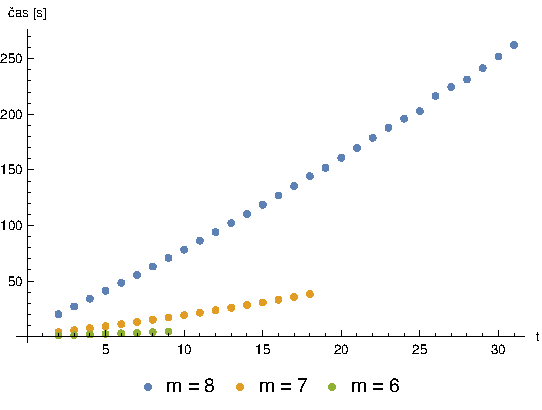
\includegraphics[width=0.7\textwidth]{../../implementace/grafy/listplot_m6-8_generovani.pdf}
        \caption[Časová složitost generování klíčů]{
            Závislost doby generování klíčů na parametru~$t$
        }
        \label{obr_mereni_t_gen}
    \end{figure}

\end{frame}

% ------------------------------------------------------------------------------
\begin{frame}{Výsledky měření}

    \begin{figure}[!ht]
        \centering
        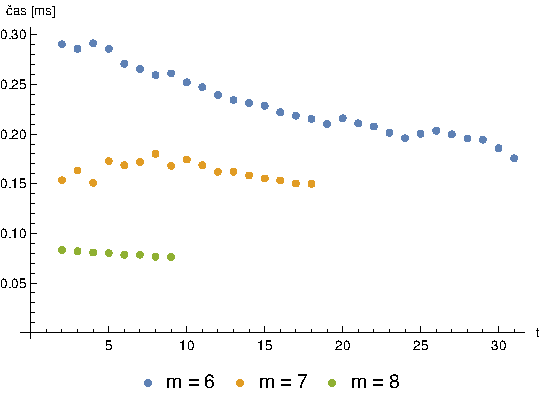
\includegraphics[width=0.7\textwidth]{../../implementace/grafy/listplot_m6-8_sifrovani.pdf}
        \caption[Časová složitost šifrování]{
            Závislost doby šifrování zprávy na parametru~$t$
        }
        \label{obr_mereni_t_sifr}
    \end{figure}

\end{frame}

% ------------------------------------------------------------------------------
\begin{frame}{Výsledky měření}

    \begin{figure}[!ht]
        \centering
        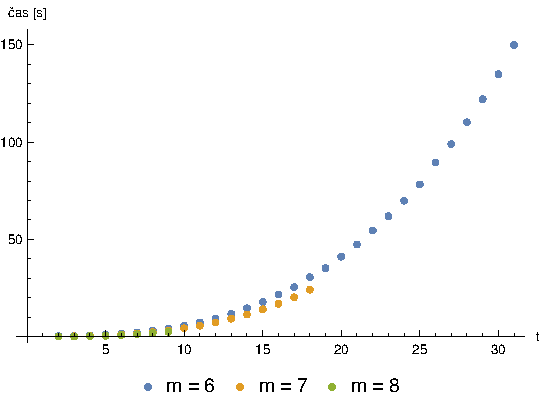
\includegraphics[width=0.7\textwidth]{../../implementace/grafy/listplot_m6-8_desifrovani.pdf}
        \caption[Časová složitost dešifrování]{
            Závislost doby dešifrování zprávy na parametru~$t$
        }
        \label{obr_mereni_t_desifr}
    \end{figure}

\end{frame}

% ------------------------------------------------------------------------------
\begin{frame}{Výsledky měření}

    \begin{figure}[!ht]
        \centering
        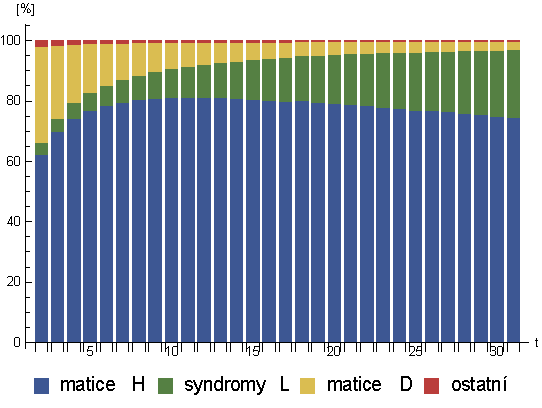
\includegraphics[width=0.7\textwidth]{../../implementace/grafy/chart_m8_generovani.pdf}
        \caption[Poměr částí výpočtu při generování klíčů]{
            Poměr významných částí výpočtu při generování klíčů v~závislosti na
            parametru~$t$ (při $m=8$)
        }
        \label{obr_mereni_pomer_gen}
    \end{figure}

\end{frame}

% ------------------------------------------------------------------------------
\begin{frame}{Výsledky měření}

    \begin{figure}[!ht]
        \centering
        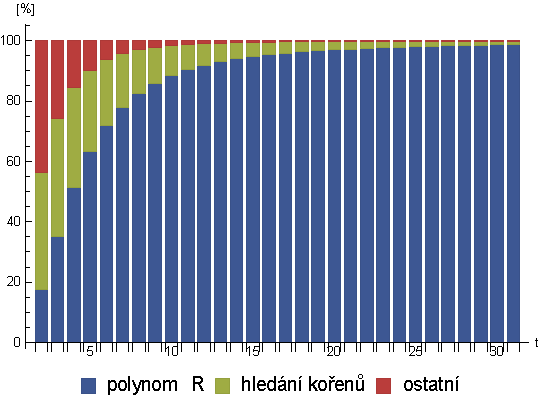
\includegraphics[width=0.7\textwidth]{../../implementace/grafy/chart_m8_desifrovani.pdf}
        \caption[Poměr částí výpočtu při dešifrování]{
            Poměr významných částí výpočtu při dešifrování zprávy v~závislosti na
            parametru~$t$ (při $m=8$)
        }
        \label{obr_mereni_pomer_desifr}
    \end{figure}

\end{frame}

%
% % ==============================================================================
% % ==============================================================================
% \section{Kryptoanalýza}
%
% % ------------------------------------------------------------------------------
% \begin{frame}{Kryptoanalýza systému McEliece}
%     \begin{alertblock}{Známé útoky na McEliece}
%         \begin{itemize}
%
%             \item Útoky na veřejný klíč
%
%                 \begin{itemize}
%                     \item \structure{Útoky na strukturu} použitého kódu
%                     \item \emph{Support Spliting Algorithm}
%                 \end{itemize}
%
%             \item Útoky na šifrový text
%                 \begin{itemize}
%                     \item Útok s~\emph{informační množinou}
%                     \item Nalezení \emph{kódového slova s~nízkou vahou}
%                         \begin{itemize}
%                             \item Algoritmus \structure{Canteaut a Chabaud}~\cite{Canteaut}
%                         \end{itemize}
%                 \end{itemize}
%
%         \end{itemize}
%     \end{alertblock}
% \end{frame}
%

% ==============================================================================
% ==============================================================================
\section{Závěr}

% ------------------------------------------------------------------------------
\begin{frame}{Závěr}
    \begin{itemize}

        \item Rešerše kryptosystému
            \begin{itemize}
                \item Základní varianta a \structure{schéma pro podpis}
                \item \structure{Kryptoanalýzy systému}
                \item Metody \structure{zkrácení klíčů} a \structure{moderní varianty}
            \end{itemize}

        \item Ukázková implementace
            \begin{itemize}
                \item Použitelné \structure{samostatné balíky}
            \end{itemize}

        \item Experimentálně ověřené složitosti
            \begin{itemize}
                \item Izolovány \structure{kritické části} výpočtu
            \end{itemize}

    \end{itemize}
\end{frame}


% ------------------------------------------------------------------------------
\begin{frame}[plain,noframenumbering]
    \begin{center}

        {
            \Large
            \structure{Děkuji za pozornost}
        }

        \vspace{1cm}

        {
            \small
            \url{https://github.com/VojtechMyslivec/mceliece-mathematica}
        }

    \end{center}
\end{frame}


% ==============================================================================
% ==============================================================================
% ==============================================================================
\appendix

% ==============================================================================
% ==============================================================================
\section{Otázky}
% ------------------------------------------------------------------------------
\begin{frame}{Otázky oponenta}
    \begin{enumerate}

        \item Má vůbec smysl hledat úsporu prostoru u~soukromého klíče,
            i~s~ohledem na vaše tvrzení, že kapacity disků jsou téměř neomezené
            a~limit je primárně v~přenosu veřejného klíče?

        \item Zkoušel jste změřit dobu generování klíčů, šifrování a~dešifrování
            pro bezpečné parametry, tedy např. $m=12$, $t=41$?

    \end{enumerate}
\end{frame}

% ------------------------------------------------------------------------------
\begin{frame}{Otázky oponenta}

    \begin{block}{1. Velikosti klíče}
        \begin{enumerate}

            \item Veřejný klíč
                \begin{itemize}
                    \item Přenos klíče
                \end{itemize}

            \item Soukromý klíč
                \begin{itemize}
                    \item Vestavěné systémy
                \end{itemize}

        \end{enumerate}
    \end{block}

\end{frame}

% ------------------------------------------------------------------------------
\begin{frame}{Otázky oponenta}
    \begin{block}{2. Rozumné parametry}

        \begin{figure}
            \centering
            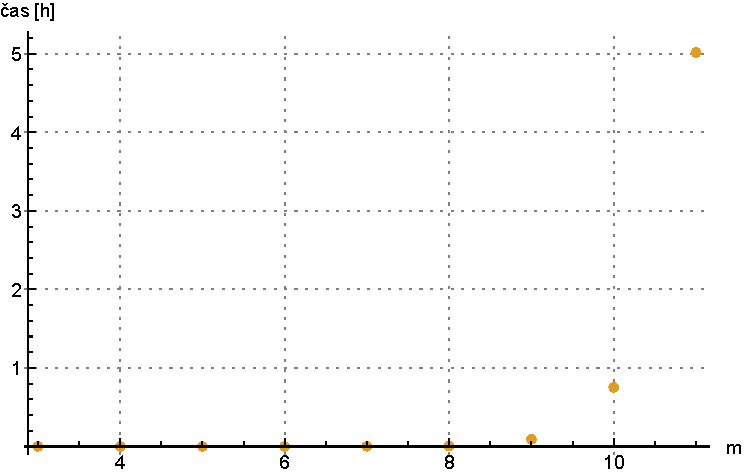
\includegraphics[width=0.7\textwidth]{../../implementace/grafy/listplot_mVelka_generovani.pdf}
            \caption[Časová složitost generování klíčů]{
                Závislost doby generování klíčů na parametru~$m$
            }
        \end{figure}

    \end{block}
\end{frame}

% % ------------------------------------------------------------------------------
% \begin{frame}{Otázky oponenta}
%     \begin{block}{2. Rozumné parametry}
%
%         \begin{figure}
%             \centering
%             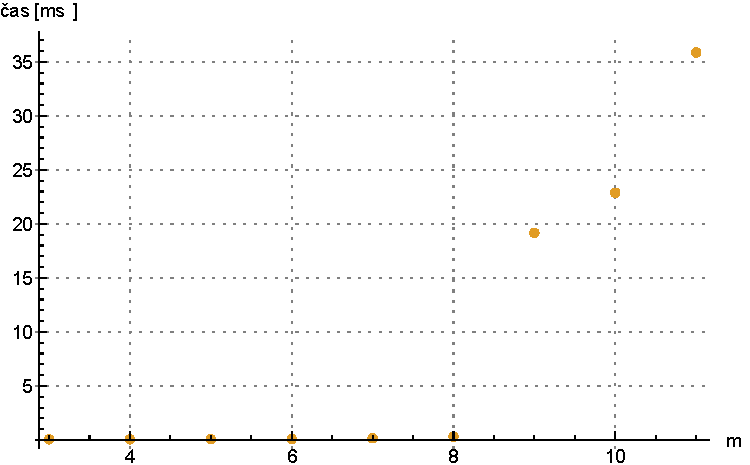
\includegraphics[width=0.7\textwidth]{../../implementace/grafy/listplot_mVelka_sifrovani.pdf}
%             \caption[Časová složitost šifrování]{
%                 Závislost doby šifrování zprávy na parametru~$m$
%             }
%         \end{figure}
%
%     \end{block}
% \end{frame}

% ------------------------------------------------------------------------------
\begin{frame}{Otázky oponenta}
    \begin{block}{2. Rozumné parametry}

        \begin{figure}
            \centering
            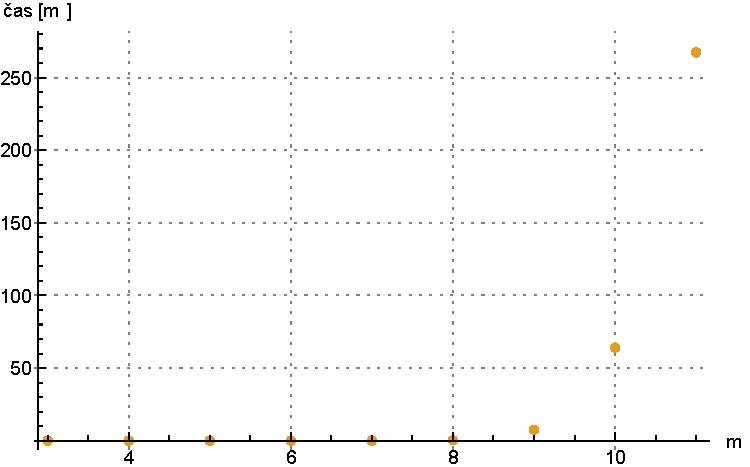
\includegraphics[width=0.7\textwidth]{../../implementace/grafy/listplot_mVelka_desifrovani.pdf}
            \caption[Časová složitost dešifrování]{
                Závislost doby dešifrování zprávy na parametru~$m$
            }
        \end{figure}

    \end{block}
\end{frame}

% ==============================================================================
% ==============================================================================
\section{Reference}
% ------------------------------------------------------------------------------
\begin{frame}[allowframebreaks]{Reference}
    \begin{thebibliography}{99}

    \bibitem{McEliece}
        Robert J. \textsc{McEliece}. A~Public-Key Cryptosystem Based on
        Algebraic Coding Theory v~\emph{JPL Deep Space Network Progress Report},
        strany 114-116. 1978. Dostupné online
        \url{http://ipnpr.jpl.nasa.gov/progress_report2/42-44/44N.PDF}

    \bibitem{Berlekamp1}
        Elwyn R. \textsc{Berlekamp}, Robert J. \textsc{McEliece}, Henk C. A. van
        \textsc{Tilborg}.  On the Inherent Intractibility v~\emph{IEEE
        Transactions of Information Theory}, vol. IT-24, No. 3, strany 384-386.
        IEEE, květen 1978.

    \bibitem{Post-Quantum_Cryptography}
        Daniel J. \textsc{Bernstein}, Johannes \textsc{Buchmann}, Erik
        \textsc{Dahmen}. \emph{Post-Quantum Cryptography}. ISBN
        978-3-540-88701-0.  Springer Berlin Heidelberg, 2009.

    \bibitem{Engelbert}
        Daniela \textsc{Engelbert}, Raphael \textsc{Overbeck}, Arthur
        \textsc{Schmidt}. A~Summary of McEliece-Type Cryptosystems and their
        Security v~\emph{Journal of Mathematical Cryptology}. IACR 2006.
        Dostupné online \url{http://eprint.iacr.org/2006/162}

    \bibitem{Goppa}
        Valery D. \textsc{Goppa}. A~New Class of Linear Correcting Codes
        v~\emph{Problemy Peredachi Informatsii}, vol. 6, strany 24-30. 1970.

    \bibitem{Paar}
        Christof \textsc{Paar}, Jan \textsc{Pelzl}. \emph{Understanding
        Cryptography}: A~Textbook for Students and Practitioners.
        Springer-Verlag Berlin Heidelberg, 2010. Dostupné
        online: \url{https://www.springer.com/us/book/9783642041006}

    \bibitem{Patterson}
        Nicholas J. \textsc{Patterson}, The algebraic decoding of Goppa codes
        v~\emph{IEEE Transactions on Information Theory}, vol. 21, strany
        203-207. IEEE 1975. Dostupné online
        \url{http://ieeexplore.ieee.org/xpl/articleDetails.jsp?arnumber=1055350}

    \bibitem{Schanck}
        J. M. Schanck, W. Whyte, Z. Zhang. Criteria for selection of public-key
        cryptographic algorithms for quantum-safe hybrid cryptography
        (Internet-draft). IETF, 2016. Dostupné online
        \url{https://datatracker.ietf.org/doc/draft-whyte-select-pkc-qsh/}

    \end{thebibliography}

\end{frame}

\end{document}
% ==============================================================================
% ==============================================================================
% ==============================================================================


